\chapter{Proposed Solution}
Ideas:
\begin{itemize}
    \item Progress
        \begin{itemize}
            \item begin flat multilayer rendering
        \end{itemize}
\end{itemize}

\section{Concepts}
\subsection{Original 2D Visualization}
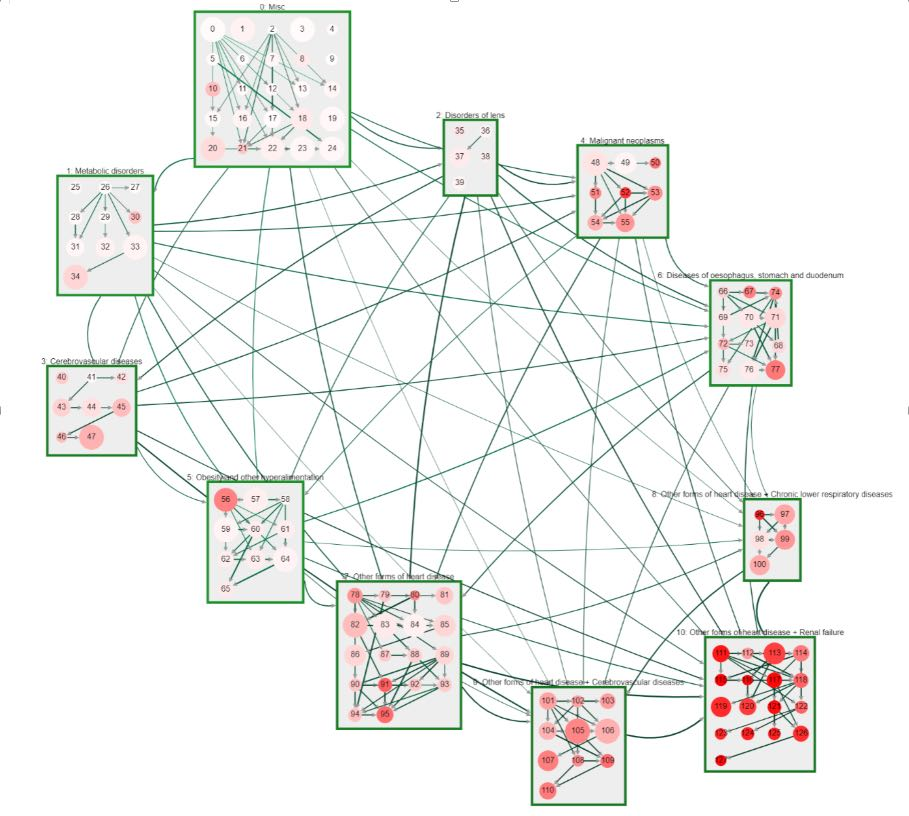
\includegraphics[width=0.5\textwidth]{chapters/graphics/2dVisOfDemoData.jpg}

Problem only two layers supported

\subsection{2-Layer Concept}
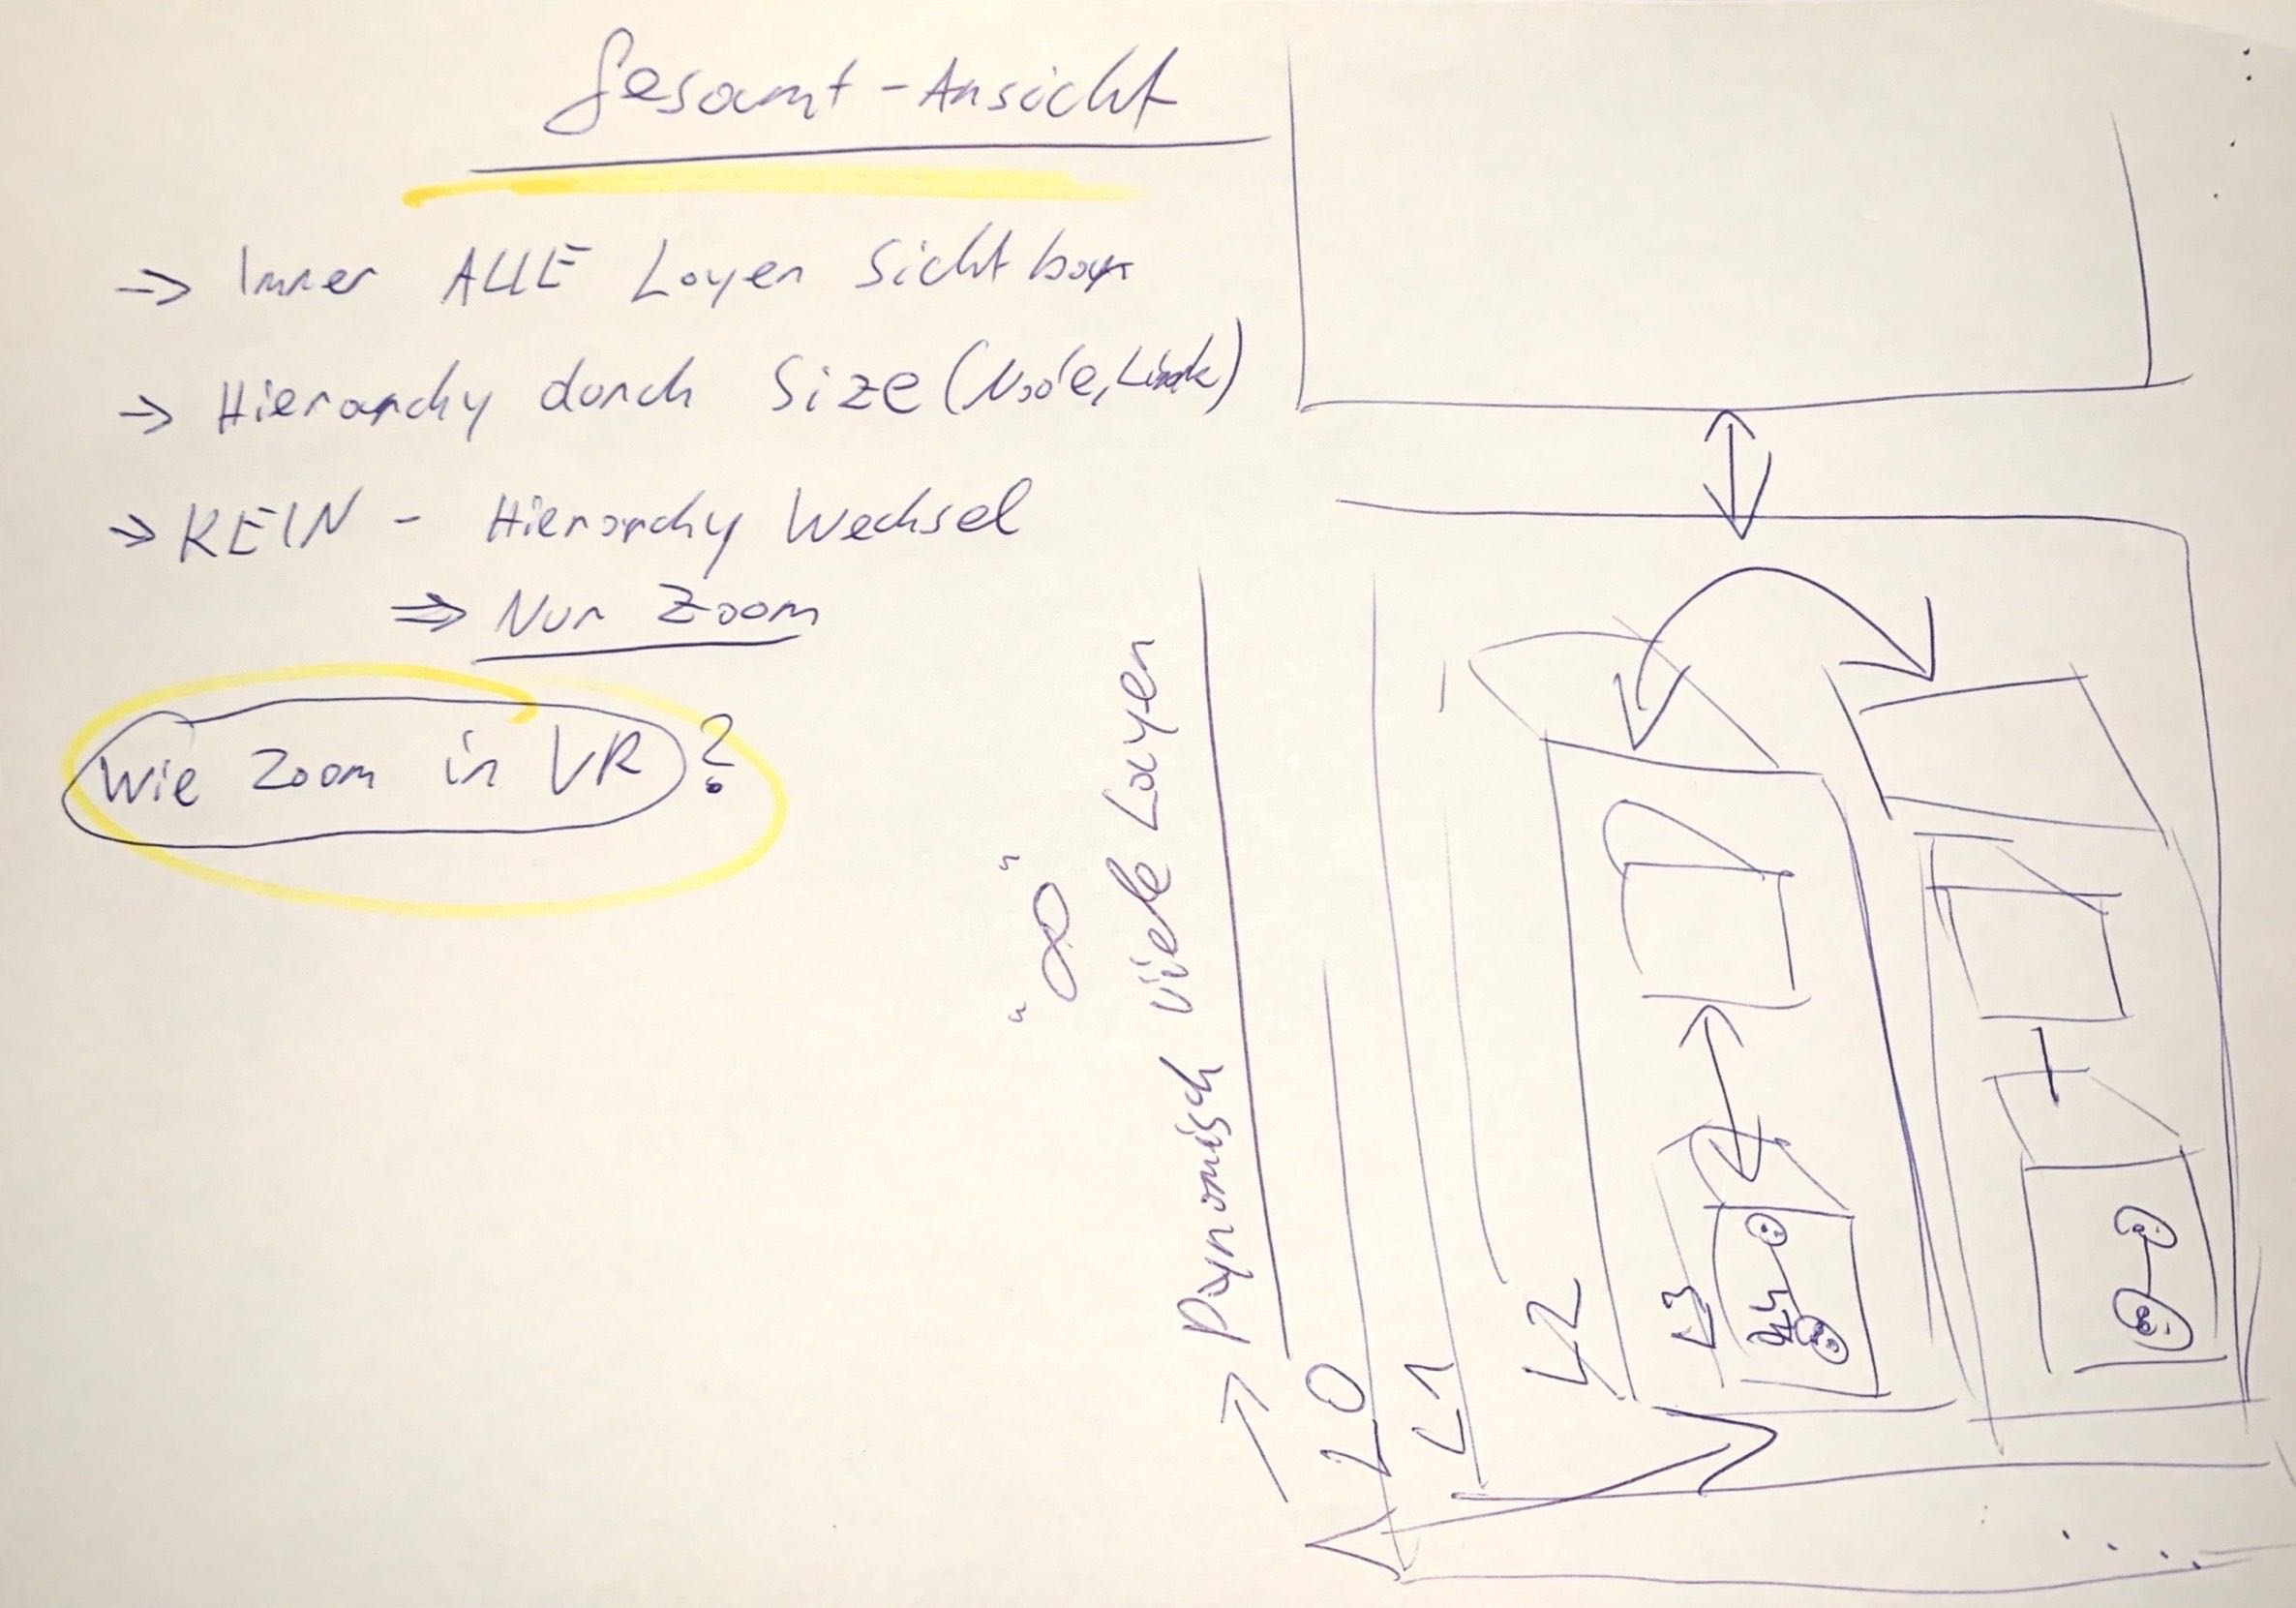
\includegraphics[width=0.5\textwidth]{chapters/graphics/concept2.jpg}

Cube/ (half) sphere position of sub-graphs \\
Starting idea, why it was discarded

\subsection{n-Layer Concept}
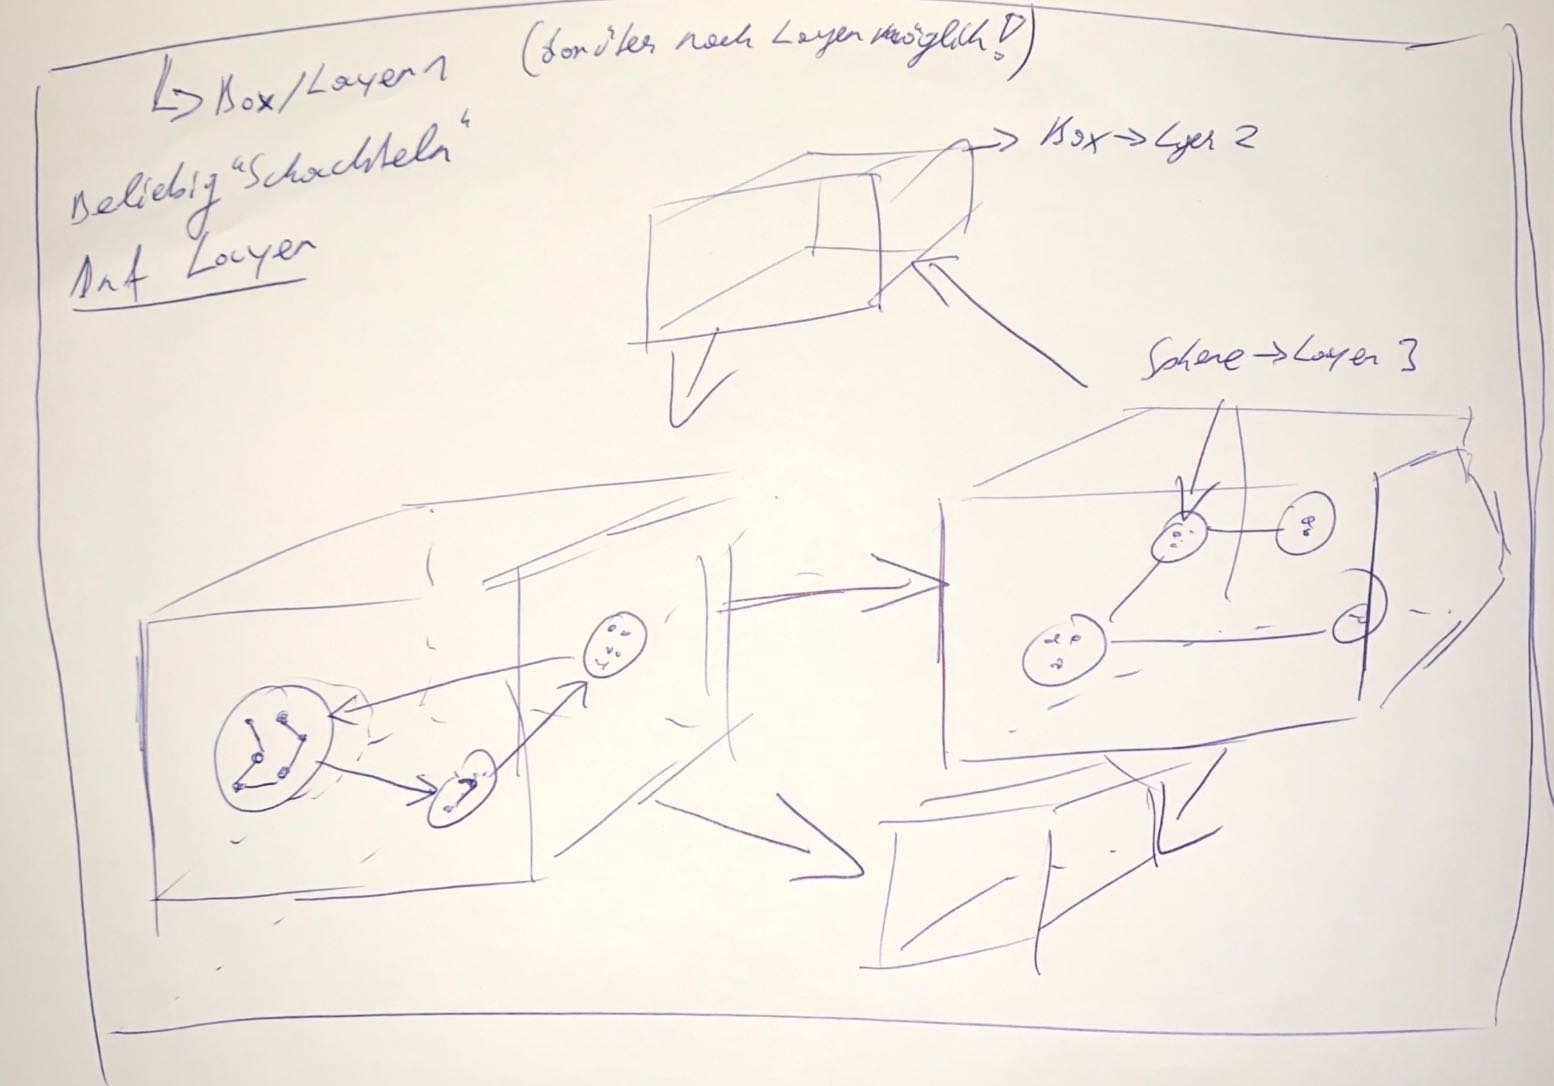
\includegraphics[width=0.5\textwidth]{chapters/graphics/concept1.jpg}

Improved concept \\
no fixed cube/(half) sphere position instead each layer calculate its own position \\
circle over boxes \\
Begin: flyspeed only, later on problem on VR \\

\section{Position of Nodes}

Independent per layer / sub-graph inside parent node \\
use of existing implemented and already good tested(prevents overlapping, good distribution, ...) forces (collision, link, manyBody, ...) \\
use of own forces to place sub-graphs inside parent graphs \\
adjustable force strengths \\
Node size grow with number of child nodes \\
\\
two possible solutions: web-worker vs live \\

\section{Usage of different Visual Features}

Position \\
linkWidth \\
linkColor \\
linkDirection \\ 
currentLayer on Controller Overlay \\ 

\section{Graph Exploration}

\subsection{Overview Layout}
Orbital Camera

\subsection{Detail Layout}
Free Fly Camera \\
change FlySpeed based on current node the camera is located. As deeper the layer as slower the flyspeed \\
Problem experiments showed this does not work well in VR --> manual / automated scaling. \\

flyToNode \\
flyToParentLayer \\

\subsection{Visibility of the Visualization}
\subsubsection{Nodes / Layers}
wireframe
\subsubsection{Links}
lockLinks

\section{Interaction}
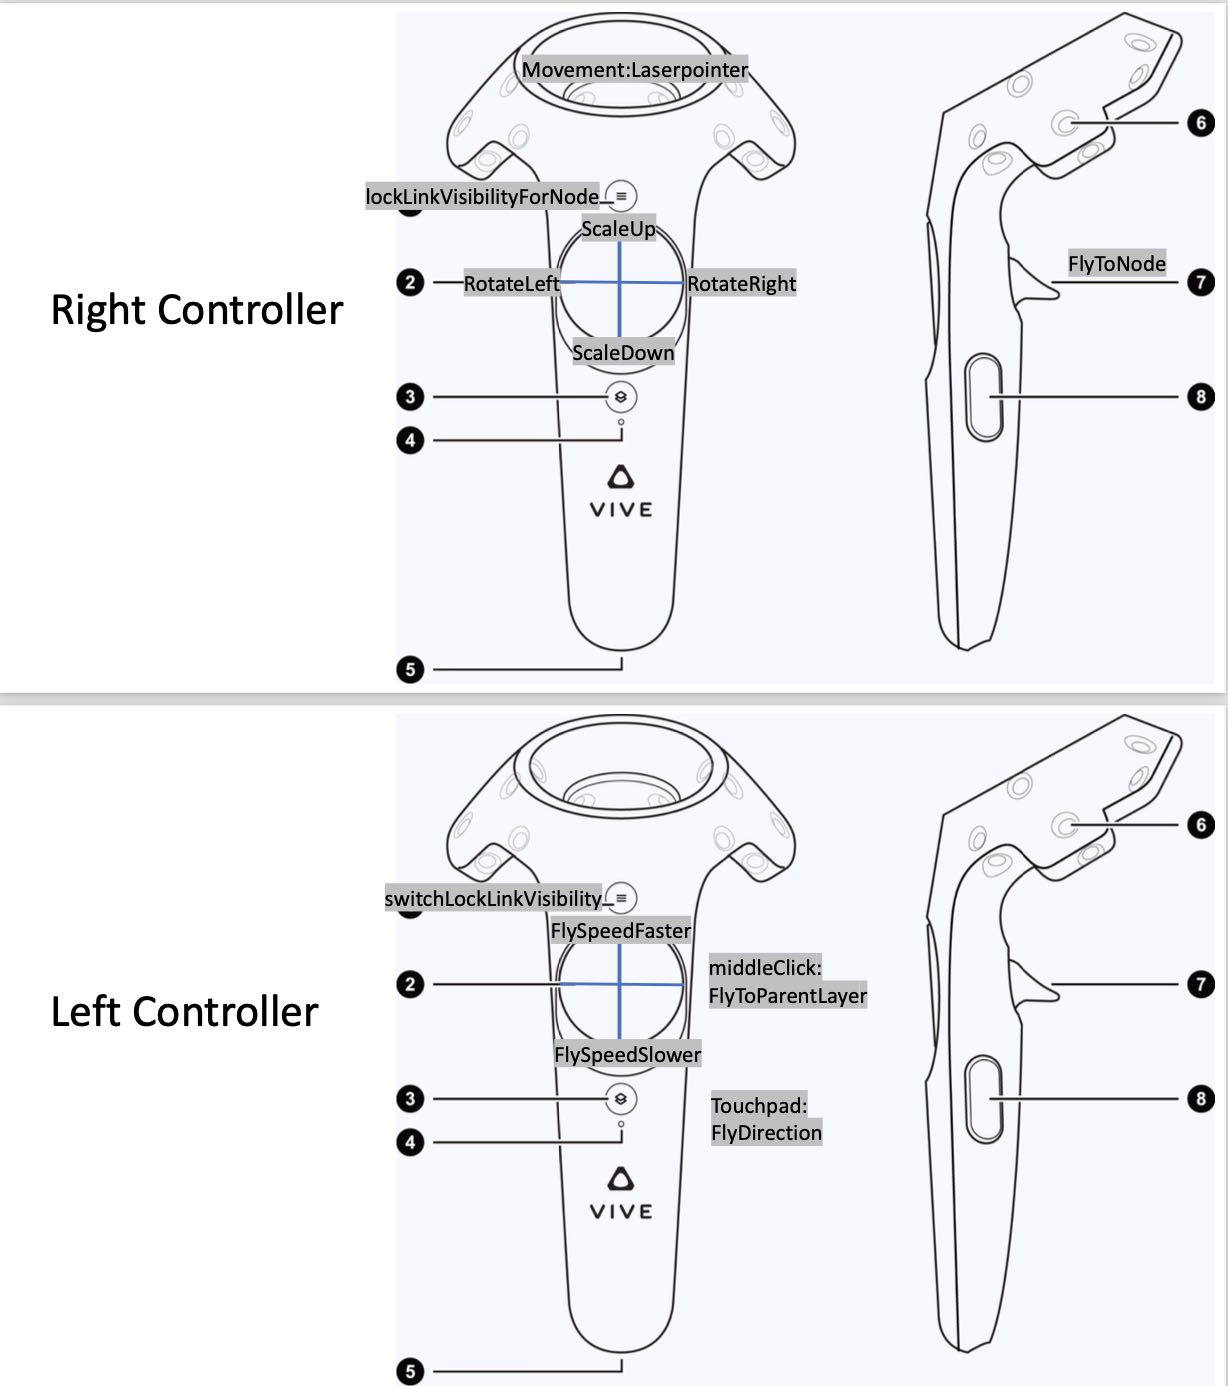
\includegraphics[width=0.5\textwidth]{chapters/graphics/controllerMapping.jpg}
